\section{Test description}
\label{section:test_description}

In this section I will describe which metrics I am going to use to compare the different algorithms. Having specified these I will describe the tests in detail.

\subsection{Metrics}

The metrics I will measure in the tests will be 
\begin{description}
\item[Number of hops:] The number of hops from the source to the sink. For this I will measure the maximum number of hops, the minimum number of hops, as well as the average. I feel the number of hops is the most important metric, since it both details how many nodes that have to expend energy before the message arrives at the node, how long it takes for the message to arrive at its destination, and how great the risk is that the network topology will make it impossible for the message to arrive (assuming, of course, that the message could arrive when it was sent).

\item[Time:] The amount of time spent sending the message from the source to the sink. I will likewise measure the maximum, minimum and average time spent. It is clear that the faster a message arrives at its sink, the better.

\item[Percentages of successfully arrived messages:] While most routing algorithms guarantees that the message will always arrive, this is not always the case . The best example of a routing algorithm that does not have this guarantee is the greedy routing algorithm (see section~\ref{section:greedy} p. \pageref{section:greedy}). Also, since we are trying to simulate mobile nodes with limited energy storage, critical parts of the topology may be fail, making it impossible for the message to arrive.
\end{description}

For the number of hops and the  amount of time I will record the maximum, the minimum and the average value. The main value for comparison will be the average value, but I feel that recording both the maximum and the minimum values will give me better information about the average.

\subsection{Input parameters}
\label{section:input_parameters}
In order to perform the tests I will need to define the parameters and their range for the different tests.
\begin{description}
\item[Movement model:] The topology is clearly going to be influenced by the way that the nodes move, therefore it would be interesting to test out several models, to see the strengths and weaknesses of the different routing algorithms.

\item[Routing Algorithms] 

\item[Amount and data-transmission type:] In real world situations there will be different levels of traffic on the network, and therefore to test it we must likewise simulate these differences. The choice of transmission protocol is also important.

\item[Size of the simulation area:] The size of the simulation area has a direct influence on how far apart the nodes can move and how many nodes are needed for a given node density. Everything else being equal, a larger simulation area will make the network less robust.

\item[Number of nodes:] It is clear that denser node distribution, everything else being equal, will give a more robust network.

\item[Percentage of nodes failing/leaving the network:] Since we are dealing with a \ac{manet}, it is clear that a nodes may leave the network or fail (either due to equipment failure or lack of power). 

\item[Percentage of nodes entering the network:] In a \ac{manet} we have to assume that nodes can enter the network.
\end{description}

\subsection{Actual parameters}
As I have now detailed in section~\ref{section:input_parameters} which parameters it would be useful to vary, I will in this subsection detail the actual value of the different parameters. 

\begin{description}
\item[Movement models:] \hide{DisasterArea \cite{disasterArea} and} Gauss-Markov \cite{MobilityAdHocResearch} with the trace created through the use of the BonnMotion tool \cite{toilers} use to create the movement files which can then be imported into ns-2\footnote{For the script that generates the movement files, please see \texttt{src/MotionCode/Gauss-Markov.py}}.
\item[Amount and Data-transmission type:] 512 kB through a TCP connection
\item[Size of simulation area:] 500 by 500 units and 1000 by 1000 units
\item[Routing algorithms:] GOAFR \cite{gopher}, GPSR \cite{gpsr}, Greedy \cite{gopher}, DSDV \cite{DSDV}
\item[Number of nodes:] 100 to 10000 nodes in increments of 100 nodes, giving me 100 data-points that will be used to analyse the success of the routing algorithms. 
%\item[Nodes failing:] 0\%, 10\%, 40\%
%\item[Nodes entering:] 0\%, 30\%
\item[Time:] 1 minute (60 seconds)
\item[Amount of nodes transmitting:] 33\% of the network
\end{description}

\subsection{Routing algorithm description}
\label{section:routing_algorithm}
In this description of the chosen routing algorithms, I will assume by default that there exists a path from the source to the sink, and if needed I will detail how the algorithm handles the cases where no such path exists.

Since I have already explained how the Greedy routing works in \ref{section:greedy}.

\subsubsection{GOAFR and GOAFR+}

GOAFR \cite{gopher} (Greedy Other Adaptive Face Routing) and GOAFR+ \cite{gopher+} (a refinement on GOAFR) are multi-stage geometrical algorithms. The algorithms are based on Greedy routing (see section~\ref{section:greedy} on p. \pageref{section:greedy}) and Adaptive Face Routing, with an adaptive ellipse $\epsilon$ as the boundary for the message. The description in the following paragraphs uses information from \cite{gopher}.

As an integral part of the algorithm, GOAFR includes an ellipsis $\epsilon$ that that the message has to keep inside, in order to avoid having the message going astray. $\epsilon$ is created so that its forci are the source $s$ and the sink $t$, and so that its semi-major axis starts out being $2 * |\overline{st}|$. Using the formula for forci
\eqa{
F = \sqrt{j^2 - n^2}
}
where $F$ is the distance from each forci to the centre, $j$ is the semi-major axis (major radius), and $n$ is semi-minor axis (minor radius) so in this case we have
\eqa{
F &=& \sqrt{j^2 - n^2}\\
\frac{|\overline{st}|}{2} &=& \sqrt{j^2 - n^2}\\
\left(\frac{|\overline{st}|}{2}\right)^2 &=& j^2 - n^2\\
n^2 &=& j^2 - \left(\frac{|\overline{st}|}{2}\right)^2\\
n &=& \sqrt{j^2 - \left(\frac{|\overline{st}|}{2}\right)^2}\\
}
which we then can use to calculate the semi-minor axis. Depending on the execution of GOAFR the major axis of $\epsilon$ might grow, as detailed in the next two paragraphs.

Having thus laid the groundwork I can now describe GOAFR:
\begin{enumerate}
\item Make the ellipsis based on the sink and the source.
\item Perform Greedy routing as described in section~\ref{section:greedy} on p. \pageref{section:greedy}. If the greedy algorithm sends the message beyond the bound of $\epsilon$, then the longest axis of $\epsilon$ is doubled. If the message arrives at the sink, then the message is handed over to the node and the algorithm terminates. If the message arrives at a local minimum (see section~\ref{section:greedy} for an explanation), go to step 3.
\item Since we have arrived at a node $u$ local minimum, we first store $u$ as both $u_{local min}$ and as $u_{closest node}$ in the message header, to indicate that it is both the node we started routing around the face as, but also the node that is closest to the sink. We then use Adaptive Face routing (which uses the right-hand rule --- see section~\ref{right-hand rule} on p. \pageref{right-hand rule}) to traverse the face, and for each node $v$ we encounter we check to see if it is closer to the sink than the current value of $u_{closest node}$, if so, we set $u_{closest node}$ to be $v$. 

If the message is about to go outside of $\epsilon$ for the first time, then the message reverses direction and the message tries to traverse the face in the other direction (skipping past $u_{local min}$) without stopping). If the message encounters $\epsilon$ for the second time, then the longest axis of $\epsilon$ is doubled and the message is forwarded as normal.

At some point the message will either arrive back at $u_{local min}$ or find the sink. If the message arrives back at $u_{local min}$ after having gone outside $\epsilon$ an even number of times, we then go to step 4. If the message arrives at the sink, then the message is handed over to the sink and the algorithm terminates.
\item The message is now forwarded to $u_{closest node}$ we found in the last step, by using the same face routing as before. Once we arrive at $u_{closest node}$ we go to step 2.
\end{enumerate}

GOAFR+ works similarly to GOAFR, with the difference being the introduction of 2 variables $p$ and $q$. While doing the adaptive face routing from the local minimum node $u_{local min}$, the algorithm keeps track of how many nodes encountered that are closer to the sink than $u_{local min}$ in the variable $p$ and how many are farther away from the sink than $u_{local min}$ in the variable $q$.
A special action is then taken if
\begin{enumerate}
\item If the message arrives at the edge of $\epsilon$ for the first time, then the message turns back and explores the face in the other direction. 
\item If the message arrives at the edge of $\epsilon$ for the second time, and no nodes have been found to be closer to the sink than $x$, then the major axis of $\epsilon$ is doubled. Otherwise the message is sent to the node closest to the sink and the greedy routing is resumed.
\item If at any point $p > \rho q$, where $\rho$ is a constant defined before routing starts, then route the message to the node closest to the sink and begin greedy routing again.
\end{enumerate}

Both GOAFR and GOAFR+ has proved to be theoretical asymptotically worst-case optimal and average-case efficient. Due to space demands I will not try to prove these claims here, but will instead refer the interested reader to \cite{gopher+, gopher}.

Due to time constraints I have only been able to implement GOAFR in ns-2, and so will only use that in the tests.

\subsubsection{GPSR}
\tikfig{gpsr}
{A demonstration of the GPSR routing algorithm. The grey background with grey nodes indicates when the GPSR algorithms is in the Greedy phase and the the black nodes with the black background indicates when the algorithm is running in perimiter phase}

\label{section:gpsr}
Greedy Perimeter Stateless Routing is a routing algorithm that uses a hybrid of Greedy routing and face routing. The idea is to use Greedy routing as much as possible, and only use the face routing recover from situations where it reaches a situation where the Greedy routing fails. The algorithm will use the right-hand-rule (see section~\ref{right-hand rule} on p. \pageref{right-hand rule}) to route the messages in perimeter mode to ensure they stay within the same face. I base all the description in this subsection on \cite{gpsr}.

If we let $x$ be the point where the Greedy routing fails, and $t$ be the sink, then the gist of the perimeter routing is to route through the faces that are intersected by the line-segment $\overline{xt}$, in order to find a point that is closer to $t$ than $x$, and possibly recover. In order to do this the algorithm will explore each face sequentially, moving on to the next face when it encounters a node or, more likely, an edge that is intersected by $\overline{xt}$. 

In order for the routing to work the algorithm relies on 4 values:
\begin{description}
\item[$t$:] The sink, which contains its own coordinates
\item[$L_p$:] The node where the algorithm went from Greedy routing to Perimeter routing. This value is overwritten if the routing goes back to Greedy routing and then back to Perimeter routing. This, together with $t$, is used to create the line-segment $\overline{L_pt}$, that is used to signal when the message is close enough to $t$ to move to the next face.
\item[$L_f$:] The point on $\overline{L_pt}$ where the message entered the current face. Most of the time this will not be the position of a node, but rather a point on an edge between the face whose perimeter the message has just explored, and the next face. 
\item[$e_0$:] The first edge the message traversed on the current face. This is used as the termination condition for the perimeter exploration in the case where $t$ is unreachable. 
\end{description}

also, in the following let $f$ denote the current face we are routing on.

\begin{enumerate}
\item The algorithm begins with greedy routing until it either reaches the sink, in which case it terminates, or it reaches a local minimum and therefore fails. In the case of failure the message enters perimeter mode and goes to step 2.
\item The message will enter perimeter routing and record its current node as both $L_p$ and $L_f$, and store the line-segment $\overline{L_pt}$, which we will use throughout our routing. The edge counter-clockwise to $L_p$ is stored in $e_0$. The algorithm goes to step 3
\item Let $p$ be the current node, if $|\overline{pt}| < |\overline{L_pt}|$ we have reached a node closer to the sink than the local minimum, and we continue with our Greedy routing --- the algorithm goes to step 1. If on the other hand $p$ is farther away from the sink than $L_p$, the message is transferred to the counter-clockwise node $q$ on $f$. If $\overline{pq} == e_0$ then we have come full circle, and there exist no path to the sink $t$, so drop the message. If on the other hand either $q$ or $\overline{pq}$ is intersected by $\overline{L_pt}$, then transmit the message to $q$ and go to step 4, otherwise just transmit the message and go to step 3.
\item Let $p$ be the current node. Set $L_f$ to $p$ and switch to the next face. Let $q$ be the counter-clockwise neighbour of $p$ on the new face and set $e_0$ to $\overline{pq}$. Go to step 3. 
\end{enumerate}

\subsubsection{DSDV}


\subsection{Mobility models}

For the mobility models I have only chosen to test Gauss-Markov, which I from \cite{MobilityAdHocResearch} found to be a good algorithm for simulating a movement pattern\footnote{Not to mention was implemented by the same team that build the Bonnmotion movement tool} that seems rather random. I would have liked to test the Disasster Area movement pattern found in \cite{disasterArea}, but I found it difficult to get the bonnMotion tool to generete the movement, as well as unsure on which defintions would create an interesting model for the different algorithms to be tested on\footnote{In order to create the a disaster area movment simulation several different zones have to be defined -- e.g. a zone for the disaster, a zone for the triage, treatment and so on.}. 

\subsection{Limited-range spanner tests}
\label{section:test_desc_spanners}
In this section I will detail how I have chosen to set up the limited-range spanner tests for the three different graphs: non-planar, the \acp{gabe} and the \acp{rng}.

\subsubsection{Creation of the graphs}
It is clear that we must create several graphs of several different number of nodes, as it otherwise is impossible to gain a proper perspective on how well the \ac{gabe} and the \ac{rng} stack up against the non-planar graph. In order to better describe the graphs I will use, I will introduce the notion of \emph{node-sets}, which is a finite set of nodes, where all nodes have a x- and y-coordinate and a transmit distance. Also of impotence is the concept of \emph{node-category}, which is a set of node-sets, where all node-sets in any given node-category has the same amount of nodes in them. 

In order to do this test I will first have to make several decisions:
\begin{itemize}
\item Decide upon whether we are going to uniformly distribute the nodes or if some sort of clustering should be done. 
\item How many node-categories I will have to create, balancing the need for data-points and their spread with the time they will take to create and analyse.
\item Decide upon the density for the node-categories --- if indeed there should be a fixed density for them, or if the density should be random.
\item The number of graph I will generate and the number of test I will perform for each graph in order to get enough test data to properly gauge the underlying data.
\end{itemize}

I have not encountered any specific point clustering algorithm in the literature besides the various mobility models (see \cite{disasterArea, MobilityAdHocResearch}) which has lead me to place the nodes uniformly in the plane. The justification of this was both the fact that part of this investigation was an experimental look into how the non-planar graph would behave compared to the \ac{gabe} and the \ac{rng}, and not just about \acp{manet}. In retrospect I can see that using data from the mobility model would proper would have given a better picture and would most likely have made it possible for me to cut down on the number of graphs that would have to have been generated (since the graphs would be representative of the the mobility model, and not just uniformly distributed). See section~\ref{section:future_work} for my recommendation for future comparisons between the graphs.   
Since I have chosen to uniformly distribute the nodes I will need a large number of tests in order for the underlying properties of the three types of graphs to emerge. Therefore I will therefore have to limit the number of node-categories so that I will be able to process all the tests. I will therefore chose to limit myself to 8 node-categories with the following number of nodes: 100, 250, 500, 1000, 2500, 5000, 7500 and 10000 nodes.

I feel this is a good compromise between having a reasonable number of data-points and big enough spread, while still being able to compute them in a reasonable amount of time. The nodes are going to be placed uniformly in the plane, with the lower bound of their coordinates being 0, and the upper bound depending on the number of points in the graph. No two points will have same the coordinates. 

Since we are dealing with limited-range spanners, the value of the node density and the radio-range of the nodes becomes important\footnote{If I had made the choice to use the mobility models or a cluster node algorithm, these factors would still have an impact, but properly less}. Different densities and radio-ranges would heavily influence the outcome of the results, as a high node density/radio-range would favour the non-planar graph over the two other graph types, while a low density/radio-range would create heavily disconnected graphs in all three cases. Since having many disconnected graphs would make testing difficult, I have tried to find combination that would give me a low number of connected components pr. node-set, while still keeping the density reasonably low. From several experiments this let me to a density of 0.01 nodes pr. square unit and a radio range of 20 units, and make the space the nodes are placed over a function of the number of nodes. Specifiably, if we let $x$ be the length of the sides in a square and $num$ be the number of nodes, then we have that the density is
\begin{eqnarray}
\frac{num}{x^2} &=& 0.01 \\
0.01 * x^2 &=& num \\
x^2 &=& 100 * num\\
x &=& \sqrt{100 * num}  
\end{eqnarray}
meaning that in practise the graphs are squares in the plane with the following dimensions, which will also be the upper limits on their coordinates:

\begin{tabular}{lrrrrrrrr}
Number of nodes: & 100 & 250 & 500 & 1000 & 2500 & 5000 & 7500 & 10000 \\
Width/height:    & 100 & 158 & 223 &  316 &  500 &  707 &  866 &  1000 
\end{tabular} 

\subsubsection{Tests to be performed}
In order to check the limited-range spanner for the three graphs, I will randomly pick two different nodes, a \emph{node-pair}, that are connected in the non-planar graph and record the shortest number of hops (the \emph{Unit distance}), as well as the shortest distance between the two nodes. I feel both values are worth finding, as the number of hops is directly applicable to \acp{manet}, while the distance is interesting from a more theoretical perspective, and will therefore also be recorded.

I will do this for all three types of graphs, and record whether or not a path exist between the node-pair in the \ac{gabe} or the \ac{rng}. If it is indeed the case that there are cases where the two alternative planar graphs removes paths, that would create an element of risk by employing them, instead of the non-planar graph.

\subsubsection{Analysis}
For each node-pair tested for the graphs I will find the total distance passed, the average distance and the average maximum and minimum distance for all the tests\footnote{I feel it is necessary to use the average since there may be outliers that easily could skew the results}. Likewise I will find the total number of hops, the average number of hops and the average maximum and minimum number of hops. Since one of the advantages of the \ac{gabe} and the \ac{rng} is that they have fewer neighbours, I will also find the total number of neighbours, the average, max- and minimum number of neighbours. I will also include the average number of connected components, which will give us an good idea of how connected the graphs are.

\subsubsection{Size of the test}
Since the node-sets that we are going to generate the graphs from are going to distributed uniformly, I feel that in order to gain a proper picture of the situation we need to generate many node-sets, so that any underlying pattern can show it self. Therefore I have decided to generate 500 different uniformly distributed node-sets. For each node-set I will then generate one non-planar graph, one \ac{gabe}, and one \ac{rng}, meaning that for each node node-category I  generate 500 graphs for the non-planar, \ac{gabe} and \ac{rng} (for a total of 1500 graphs for each - except for node-category 7500 and 10000, for which I only have been able to generate 250 for each, due to time constraints). Each node-set is then used to generate the three types of graph. For each node-set I then generate 100 node-pairs. I feel that this will give me an reasonable amount of data to analyse, while still being computable for the larger number of nodes.



\hide{
%\tikgraph{avg_neigh}{caption}

\begin{figure}
\centering
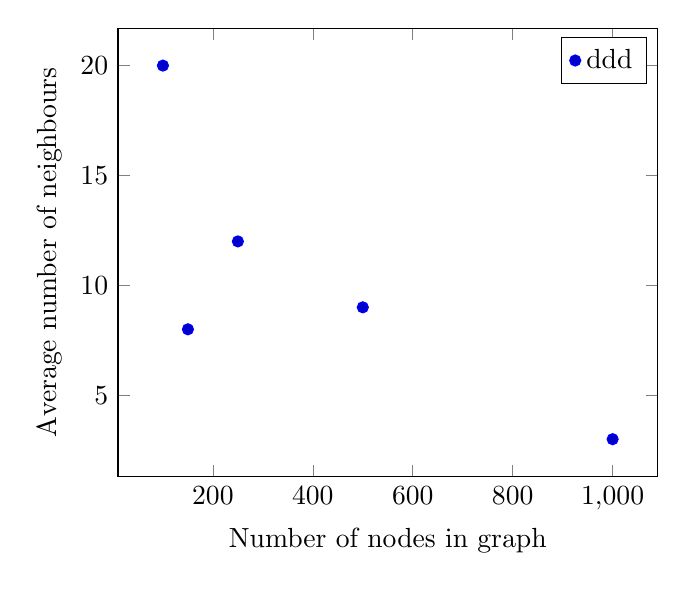
\begin{tikzpicture}
\begin{axis}[xlabel=Number of nodes in graph, ylabel=Average number of neighbours]
\addplot+[only marks] coordinates{
(100, 20) (150, 8) (250, 12) (500, 9) (1000, 3)
};
\legend{ddd}
\end{axis}
\end{tikzpicture}
\caption{Example}
\end{figure}


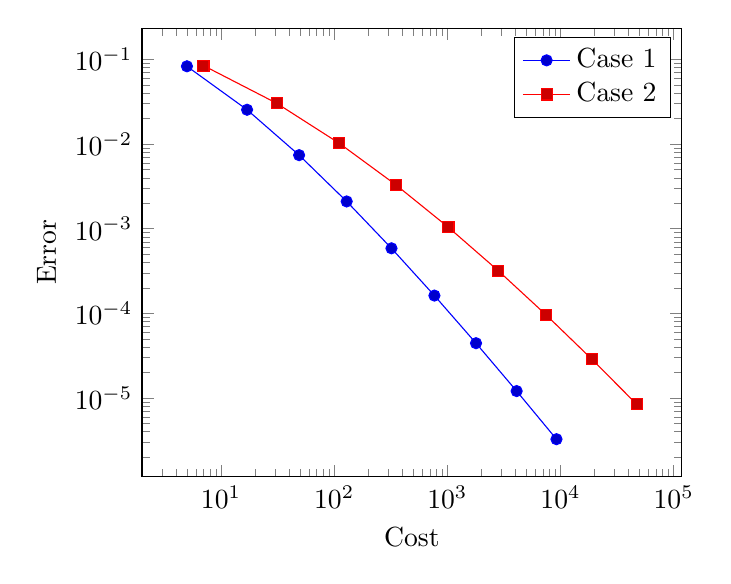
\begin{tikzpicture}
\begin{loglogaxis}[xlabel=Cost,ylabel=Error]

\addplot coordinates {
(5,
8.31160034e-02)
(17,
2.54685628e-02)
(49,
7.40715288e-03)
(129,
2.10192154e-03)
(321,
5.87352989e-04)
(769,
1.62269942e-04)
(1793, 4.44248889e-05)
(4097, 1.20714122e-05)
(9217, 3.26101452e-06)
};
\addplot coordinates {
(7,
8.47178381e-02)
(31,
3.04409349e-02)
(111,
1.02214539e-02)
(351,
3.30346265e-03)
(1023, 1.03886535e-03)
(2815, 3.19646457e-04)
(7423, 9.65789766e-05)
(18943, 2.87339125e-05)
(47103, 8.43749881e-06)
};
\legend{Case 1,Case 2}
\end{loglogaxis}
\end{tikzpicture}
\caption{A larger example}
\end{figure}
}
